\index{Foundation}
FoundationモジュールはすべてのSpringheadクラスの基本クラスを定義します.
\KLUDGE 普通に使っている限り,ユーザがFoundationの機能を直接利用することは少ないでしょう.

\section{実行時型情報}

\index{IfInfo}
\KLUDGE (ほとんど)すべてのSpringheadオブジェクトは実行時型情報(RTTI)を持っています.
C++にも\texttt{dynamic\_cast}などのRTTI機能がありますが,これよりも大幅にリッチな型情報が提供されます.

\KLUDGE 実行時型情報のクラスは\texttt{IfInfo}です.
\texttt{IfInfo}は次節で紹介する\texttt{Object}クラスから取得できます.

\section{オブジェクト}

\begin{figure}[t]
\begin{center}
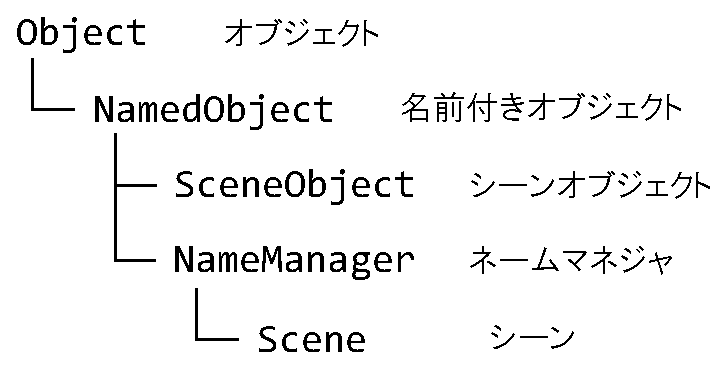
\includegraphics[width=.5\hsize]{fig/utclass.eps}
\end{center}
\caption{Object class hierarchy}
\label{fig_utclass}
\end{figure}

\index{Object}
\KLUDGE ほとんどすべてのSpringheadオブジェクトは\texttt{Object}クラスから派生します.
\KLUDGE オブジェクトは複数の子オブジェクトを持つことができます.
Springheadのデータ構造はオブジェクトが成すツリー構造によって出来上がっています.
Foundationモジュールにおける\texttt{Object}からのクラス階層をFig.\,\ref{fig_utclass}に示します.

\KLUDGE まず\texttt{Object}クラスの子オブジェクトの作成・管理に関係する関数を紹介します.

\noindent
\begin{tabular}{p{1.0\hsize}}
\\
\texttt{ObjectIf}										\\ \midrule
\texttt{size\_t NChildObject()}							\\
\KLUDGE 子オブジェクトの数を取得する.							\\
														\\
\texttt{ObjectIf* GetChildObject(size\_t pos)}			\\
\texttt{pos}番目の子オブジェクトを取得する.			\\
														\\
\texttt{bool AddChildObject(ObjectIf* o)}				\\
\KLUDGE オブジェクト\texttt{o}を子オブジェクトとして追加する.
\KLUDGE 正しく追加されたら\texttt{true},それ以外は\texttt{false}を返す.\\
														\\
\texttt{bool DelChildObject(ObjectIf* o)}				\\
\KLUDGE オブジェクト\texttt{o}を子オブジェクトから削除する.
\KLUDGE 正しく削除されたら\texttt{true},それ以外は\texttt{false}を返す.\\
														\\
\texttt{void Clear();}									\\
\KLUDGE クリアする.												\\
\\
\end{tabular}

\KLUDGE これらの関数は派生クラスによって実装されますので,追加できる子オブジェクトの種類や数などはクラスごとに異なります.
\KLUDGE また,Springheadを普通に使用する範囲内ではユーザがこれらの関数を直接呼び出す場面はないでしょう.

\KLUDGE ストリーム出力のために以下の機能があります.

\noindent
\begin{tabular}{p{1.0\hsize}}
\\
\texttt{ObjectIf}										\\ \midrule
\texttt{void Print(std::ostream\& os) const}			\\
\KLUDGE オブジェクトの内容をストリーム\texttt{os}に出力する.	\\
\\
\end{tabular}
\texttt{Print}は,基本的にはそのオブジェクトの名前を出力し,子オブジェクトの\texttt{Print}を再帰的に呼び出します.
\KLUDGE ただし派生クラスによって\texttt{Print}で出力される内容がカスタマイズされている場合はその限りではありません.

\texttt{NamedObject}は名前付きオブジェクトです.
\texttt{NamedObject}の派生クラスには名前を文字列で与えることができ,名前からオブジェクトを検索することができます.
\KLUDGE 名前付きオブジェクトには,直接の親オブジェクト以外に,名前を管理するためのネームマネジャが対応します.

\noindent
\begin{tabular}{p{1.0\hsize}}
\\
\texttt{NamedObjectIf}									\\ \midrule
\texttt{const char* GetName()}			\\
\KLUDGE 名前を取得する.						\\
\\
\texttt{void SetName(const char* n)}	\\
\KLUDGE 名前を設定する.						\\
\\
\texttt{NameManagerIf* GetNameManager()}	\\
\KLUDGE ネームマネジャを取得する.					\\
\\
\end{tabular}

\KLUDGE 名前付きオブジェクトからはさらにシーンオブジェクトが派生します.
\KLUDGE シーンオブジェクトからは周辺モジュールのオブジェクト(\texttt{PHSolid}, \texttt{GRVisual}など)が派生します.

\noindent
\begin{tabular}{p{1.0\hsize}}
\\
\texttt{SceneObjectIf}					\\ \midrule
\texttt{SceneIf* GetScene()}			\\
\KLUDGE 自身が所属するシーンを取得する.		\\
\\
\end{tabular}

\section{ネームマネジャとシーン}

\index{NameManager}
\KLUDGE ネームマネジャは名前付きオブジェクトのコンテナとして働き,それらの名前を管理します.
\KLUDGE また,ネームマネジャはそれ自身名前付きオブジェクトです.

\noindent
\begin{tabular}{p{1.0\hsize}}
\\
\texttt{NameManagerIf}									\\ \midrule
\texttt{NamedObjectIf* FindObject(UTString name)}		\\
\KLUDGE 名前が\texttt{name}のオブジェクトを検索し,見つかればそのオブジェクトを返す.
\KLUDGE 見つからなければ\texttt{NULL}を返す.					\\
\\
\end{tabular}


\index{Scene}
\KLUDGE シーンはシーンオブジェクトのコンテナです.
\KLUDGE シーンの基本クラスは\texttt{Scene}で,ここから各モジュールのシーン(\texttt{PHScene}, \texttt{GRScene}, \texttt{FWScene}など)が派生します.
\texttt{Scene}クラスは特に機能を提供しません.


\section{タイマ}
\label{sec_uttimer}

\index{UTTimer}
\index{たいま@タイマ}
\KLUDGE タイマ機能もFoundationで提供されます.
\KLUDGE タイマクラスは\texttt{UTTimer}です.
\KLUDGE タイマを作成するには
\begin{sourcecode}
UTTimerIf* timer = UTTimerIf::Create();
\end{sourcecode}
\KLUDGE とします.\texttt{UTTimer}には以下のAPIがあります.
\begin{center}
\begin{tabular}{ll}
\texttt{[Get|Set]Resolution}		& 分解能の取得と設定	\\
\texttt{[Get|Set]Interval}			& 周期の取得と設定		\\
\texttt{[Get|Set]Mode}				& モードの取得と設定	\\
\texttt{[Get|Set]Callback}			& コールバック関数の取得と設定 \\
\texttt{IsStarted}					& 動いているかどうか	\\
\texttt{IsRunning}					& コールバック呼び出し中 \\
\texttt{Start}						& 始動	\\
\texttt{Stop}						& 停止	\\
\texttt{Call}						& コールバック呼び出し
\end{tabular}
\end{center}
\texttt{SetMode}で指定できるモードには以下があります.
\begin{center}
\begin{tabular}{ll}
\texttt{MULTIEDIA}		& マルチメディアタイマ			\\
\texttt{THREAD}		& 独立スレッド					\\
\texttt{FRAMEWORK}		& Frameworkが提供するタイマ		\\
\texttt{IDLE}			& Frameworkが提供するアイドルコールバック
\end{tabular}
\end{center}
\KLUDGE マルチメディアタイマはWindowsが提供する高機能タイマです.
\KLUDGE 独立スレッドモードでは,タイマ用のスレッドが実行され\texttt{Sleep}関数により周期が制御されます.
\texttt{FRAMEWORK}と\texttt{IDLE}モードを利用するには\texttt{FWApp}の\texttt{CreateTimer}関数を用いる必要があります.
\KLUDGE 基本的に\texttt{FRAMEWORK}モードではGLUTのタイマコールバックが使われ,
\texttt{IDLE}モードではGLUTのアイドルコールバックが使われます.

Frameworkモジュールの\texttt{FWApp}を利用する場合は,\texttt{FWApp}の\texttt{CreateTimer}関数を利用する方が便利でしょう.


\section{状態の保存・再現}
\KLUDGE シミュレーションを行うと、シーンを構成するオブジェクトの状態が変化する。
\KLUDGE ある時刻での状態を保存しておき、再現することができると、数ステップ前に戻ったり、あるステップのシミュレーションを、力を加えた場合と加えない場合で比べたりといった作業ができる。
Springheadでは、\texttt{ObjectStatesIf}を用いることで、以下のようにシーン全体の状態をまとめてメモリ上に保存、再現することができる。

\begin{sourcecode}
	PHSceneIf* phScene;
\KLUDGE 	省略:phScene(物理シミュレーションのシーン)の構築
	UTRef<ObjectStatesIf> states;
	states = ObjectStatesIf::Create();	// ObjectStatesオブジェクトの作成
	states->AllocateState(phScene);		// 保存用のメモリ確保
	states->SaveState(phScene);			// 状態の保存
	phScene->Step();					// 仮のシミュレーションを進める
\KLUDGE 	省略:加速度の取得など
	states->LoadState(phScene);			// 状態の再現
	states->ReleaseState();				// メモリの開放
\KLUDGE 	省略:力を加えるなどの処理
	phScene->Step();					// 本番のシミュレーションを進める
\end{sourcecode}

\subsection{保存・再現のタイミング}
Springheadのシーン(PHSceneやCRScene)は、複数のエンジン(PHEngineやCREngineの派生クラス)を呼び出すことで、シミュレーションを進める。
\KLUDGE シーンは、エンジンの呼び出し中以外のタイミングであればいつでも状態を保存・再現することができる。

\subsection{シーン構成変更の制約}
\KLUDGE 状態保存用のメモリは、シーンの構成に依存している。\texttt{AllocateState(), SaveState(), LoadState()}だけでなく、\texttt{ObjectStatesIf::ReleaseState()}も依存するので、\texttt{ObjectIf::AddChildObject()}などのAPIによってシーンの構成を変化させてしまうと、保存・再現だけでなくメモリの開放もできなくなる。変更前に開放するか、シーン構成を戻してから開放する必要がある。
